%%%%%%%%%%%%%%%%%%%%%%%%%%%%%%%%%%%%%%%%%%%%%%%%%%%%%%%%%%%%%%%%%%%%%%%%%%%%%%%%
%2345678901234567890123456789012345678901234567890123456789012345678901234567890
%        1         2         3         4         5         6         7         8



\documentclass[letterpaper, 10 pt, conference]{ieeeconf}\usepackage[]{graphicx}\usepackage[]{color}
%% maxwidth is the original width if it is less than linewidth
%% otherwise use linewidth (to make sure the graphics do not exceed the margin)
\makeatletter
\def\maxwidth{ %
  \ifdim\Gin@nat@width>\linewidth
    \linewidth
  \else
    \Gin@nat@width
  \fi
}
\makeatother

\definecolor{fgcolor}{rgb}{0.345, 0.345, 0.345}
\newcommand{\hlnum}[1]{\textcolor[rgb]{0.686,0.059,0.569}{#1}}%
\newcommand{\hlstr}[1]{\textcolor[rgb]{0.192,0.494,0.8}{#1}}%
\newcommand{\hlcom}[1]{\textcolor[rgb]{0.678,0.584,0.686}{\textit{#1}}}%
\newcommand{\hlopt}[1]{\textcolor[rgb]{0,0,0}{#1}}%
\newcommand{\hlstd}[1]{\textcolor[rgb]{0.345,0.345,0.345}{#1}}%
\newcommand{\hlkwa}[1]{\textcolor[rgb]{0.161,0.373,0.58}{\textbf{#1}}}%
\newcommand{\hlkwb}[1]{\textcolor[rgb]{0.69,0.353,0.396}{#1}}%
\newcommand{\hlkwc}[1]{\textcolor[rgb]{0.333,0.667,0.333}{#1}}%
\newcommand{\hlkwd}[1]{\textcolor[rgb]{0.737,0.353,0.396}{\textbf{#1}}}%

\usepackage{framed}
\makeatletter
\newenvironment{kframe}{%
 \def\at@end@of@kframe{}%
 \ifinner\ifhmode%
  \def\at@end@of@kframe{\end{minipage}}%
  \begin{minipage}{\columnwidth}%
 \fi\fi%
 \def\FrameCommand##1{\hskip\@totalleftmargin \hskip-\fboxsep
 \colorbox{shadecolor}{##1}\hskip-\fboxsep
     % There is no \\@totalrightmargin, so:
     \hskip-\linewidth \hskip-\@totalleftmargin \hskip\columnwidth}%
 \MakeFramed {\advance\hsize-\width
   \@totalleftmargin\z@ \linewidth\hsize
   \@setminipage}}%
 {\par\unskip\endMakeFramed%
 \at@end@of@kframe}
\makeatother

\definecolor{shadecolor}{rgb}{.97, .97, .97}
\definecolor{messagecolor}{rgb}{0, 0, 0}
\definecolor{warningcolor}{rgb}{1, 0, 1}
\definecolor{errorcolor}{rgb}{1, 0, 0}
\newenvironment{knitrout}{}{} % an empty environment to be redefined in TeX

\usepackage{alltt}  % Comment this line out
                                                          % if you need a4paper
%\documentclass[a4paper, 10pt, conference]{ieeeconf}      % Use this line for a4
                                                          % paper

\IEEEoverridecommandlockouts                              % This command is only
                                                          % needed if you want to
                                                          % use the \thanks command
\overrideIEEEmargins
% See the \addtolength command later in the file to balance the column lengths
% on the last page of the document



% The following packages can be found on http:\\www.ctan.org
%\usepackage{graphics} % for pdf, bitmapped graphics files
%\usepackage{epsfig} % for postscript graphics files
%\usepackage{mathptmx} % assumes new font selection scheme installed
%\usepackage{times} % assumes new font selection scheme installed
%\usepackage{amsmath} % assumes amsmath package installed
%\usepackage{amssymb}  % assumes amsmath package installed

\title{\LARGE \bf
Predictive modeling for house price prediction
}

%\author{ \parbox{3 in}{\centering Huibert Kwakernaak*
%         \thanks{*Use the $\backslash$thanks command to put information here}\\
%         Faculty of Electrical Engineering, Mathematics and Computer Science\\
%         University of Twente\\
%         7500 AE Enschede, The Netherlands\\
%         {\tt\small h.kwakernaak@autsubmit.com}}
%         \hspace*{ 0.5 in}
%         \parbox{3 in}{ \centering Pradeep Misra**
%         \thanks{**The footnote marks may be inserted manually}\\
%        Department of Electrical Engineering \\
%         Wright State University\\
%         Dayton, OH 45435, USA\\
%         {\tt\small pmisra@cs.wright.edu}}
%}
\author{Minsu Kim, Lingjie Qiao, Kevin Liao, Cheng Peng \\
University of California at Berkeley} %
\IfFileExists{upquote.sty}{\usepackage{upquote}}{}
\begin{document}

\maketitle
\thispagestyle{empty}
\pagestyle{empty}


%%%%%%%%%%%%%%%%%%%%%%%%%%%%%%%%%%%%%%%%%%%%%%%%%%%%%%%%%%%%%%%%%%%%%%%%%%%%%%%%
\begin{abstract}

This paper summarizes the background, problem, methodology and results of our analysis on predicting house price in Ames, Iowa. To make full use of statistical models and machine learning techniques we have learned from Stats 159 Reproducible and Collaborative Statistical Data Science, we participate in Kaggle Competition, \textbf{"House Price: Advanced Regression Techniques"}. We use the Ames Housing dataset compiled by Dean De Cock for use in data science education. While the competition only emphasizes the accuracy of predicted values, this paper elaborates thorough explanations on exploratory analysis, feature engineering and statistical modeling. Furthermore, we put our effort on reproducibility of this analysis, so that the reader can reproduce the exact same result from our code.

\end{abstract}


%%%%%%%%%%%%%%%%%%%%%%%%%%%%%%%%%%%%%%%%%%%%%%%%%%%%%%%%%%%%%%%%%%%%%%%%%%%%%%%%
\section{INTRODUCTION}

The House Price project thoroughly explores the predictive modeling process and advanced regression techniques. From previous study, in order to understand the relationship of one dependent variable with several independent variables, we fit a multiple linear regession with Ordinary Least Squares. However, since OLS may have high variance and include irrelevant variables, Predictive Modeling Process can improve the results in terms of Prediction Accuracy and Model Interpretability.

The competition sets the background of the project: Ask a home buyer to describe their dream house, and they probably won't begin with the height of the basement ceiling or the proximity to an east-west railroad. But this playground competition's dataset proves that much more influences price negotiations than the number of bedrooms or a white-picket fence. 

With 79 explanatory variables describing (almost) every aspect of residential homes in Ames, Iowa, this competition requires participants to predict the final price of each home. Our team therefore follows the idea of model prediction and tries to use different techniques in order to most accurately predict the final sales price of each house.

\section{DATA DESCRIPTION}
The datasets are obtained from the Kaggle Competition website. We have access to four files: 
\begin{itemize}
\item \textit{data description}, which provides the official definition for fields.
\item \textit{train.csv}, which provides 1459 real observations that can be used for model construction.
\item \textit{test.csv}, which is used to fit the predictive model and create submission entry for the final sales price of 1460 observations 
\item \textit{sample submission}, which gives an example of how the fitted values should be submitted.
\end{itemize}

The train dataset has in total 80 variables, 79 predictors and 1 target variable called \textit{SalePrice}. We observe both categorial predictors, such as \textit{FireplaceQu}, \textit{GarageCond} and \textit{MasVnrType} as well as numerical predictors, such as \textit{PoolArea}, \textit{EnclosedPorch} and \textit{YrSold}. Since we can potentially create a lot of different new variables, our goal is to understand the relationship between \textit{SalePrice} and these predictors with statistical fitting procedures that minimizes Mean Square Error.

\section{EXPLORATORY DATA ANALYSIS}
In order to choose the model to accurately predict the housing price, we first need to understand the provided dataset by conducting exploratory data analysis (aka EDA). Separating categorical predictors and numerical predictors, we can explore in two perspectives: 1) the distribution of varible itself, and 2) the relationship between explanatory variable and response variable. 
   \begin{figure}[thpb]
      \centering
      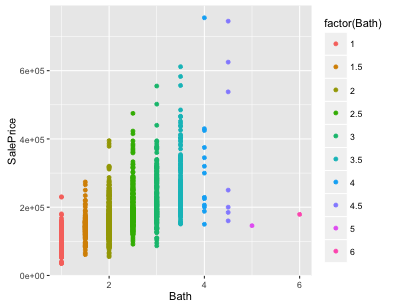
\includegraphics[width =  9cm, height = 5cm]{../images/eda-bath-vs-sale.png}
      \caption{Exploratory Data Analysis - Relationship Between Bath and SalePrice}
      \label{figurelabel}
   \end{figure}
   
   \begin{figure}[thpb]
      \centering
      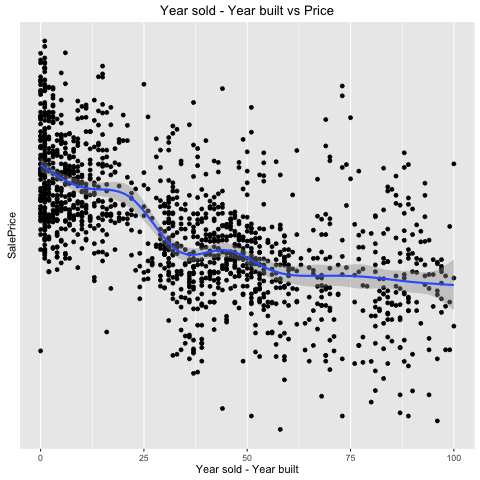
\includegraphics[width =  4cm, height = 4.5cm]{../images/scatter_Year_sold_Year_built_Vs_Price.png}
      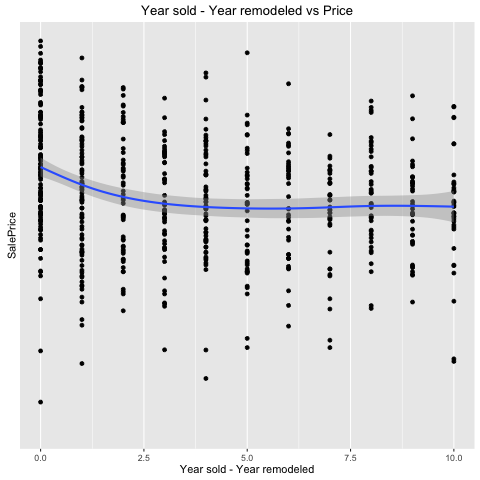
\includegraphics[width =  4cm, height = 4.5cm]{../images/scatter_Year_sold_Year_remodeled_Vs_Price.png}
      \caption{Exploratory Data Analysis - scatter plot of year sold - year built vs. sale price as well as year sold - year remodeled vs sale price}
      \label{figurelabel}
   \end{figure}
   
Figure 1 is an example of explanatory data analysis, which presents the relationship between explanatory variable bath and the response variable SalePrice. Figure 2 is a more complicated yet informative plot, which shows the relationship between sales price and the difference of year sold and year built, namely the age of house after being built, as well as the difference of year sold and year remodeled, namely the age of house after being remodeled.

Some interesting observations we made include: 1) While some variables are equally distributed in their own segments, some variables are skewed in certain directions (either to the left or to the right), which means some potential data transformation can be made to improve the predictive model; 2) We observe some linear relationship between variables, which can be used in the future model selection; and 3) While some variables have strong linear relationship with the response variable SALEPRICE, other variables do not display the similar pattern. This might encourage us to remove unnecessary predictors from the dataset in terms of model fitting and selecting.

\section{METHODOLOGY}

The goal of this analysis is to accurately predict the final price of each home. Therefore, we frame this problem as a regression problem, and decide to use the L2 loss function [1] which is often used in regression problem. Taking this objective into account, we preprocess original dataset so that regression models can work well. Furthermore, we extract more features by involving feature engineering. Finally, we fit two shrinkage models and two ensemble models. The details are explained in the following subsections.

\subsection{Evaluation and objective loss function}

We specifically use root mean squared logarithmic error [2], which makes more sense in our problem setting because errors in predicting expensive houses and cheap houses should affect the result equally. The following is the formula of RMSLE.

$$
\epsilon = \sqrt{\frac{1}{n} \sum_{i=1}^{n} (log(p_{i} + 1) - log(a_{i} + 1))^2}
$$

Since L2 loss function minimizes the squared differences between the estimated and existing target values [1], L2 error will be much larger in the case of outlier compared to L1 and therefore L2 loss function is highly sensitive to outliers in the dataset. So, in the preprocessing step, we eliminate outliers to remedy this issue.

\subsection{Preprocess}
According to the exploratory data analysis, we find a lot of NA values in most of predictors. Since regression models cannot handle missing data, we need to either remove or impute data using appropriate methods [3]. The data description provided by client [4] indicates that some of the missing values are actually none value. In that case, we replace NA value with factor variable named None. However, there are some numerical predictors with missing values in an unsystematical manner. In that case, we impute them with mean values of predictors.

As a next step, we apply log transformations to area related predictors such as GrLivArea and LotArea as well as target variable. The log transformation has an effect to remedy skewness of data [5] by making original distributions of predictors to more normally distributed. Consequently, it helps regression model to work better.

   \begin{figure}[thpb]
      \centering
      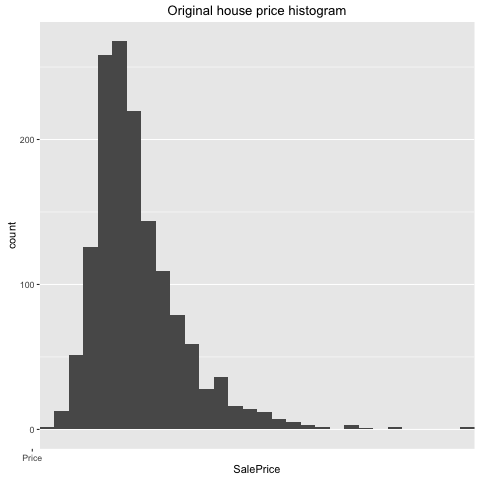
\includegraphics[width =  4cm, height = 4cm]{../images/historgram_original_price.png}
      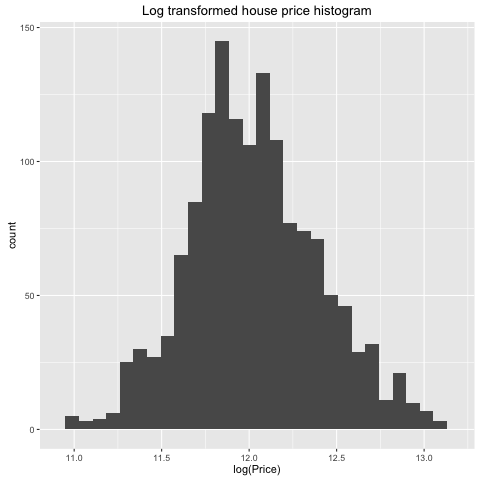
\includegraphics[width =  4cm, height = 4cm]{../images/historgram_log_trasformed_price.png}
      \caption{Effect of Log Transformation - the distribution of original sale price and the distribution of sales price after log transformation}
      \label{figurelabel}
   \end{figure}
   
After the log transformation, we still notice few outliers and eliminate lowest and highest 0.1\% data points. Furthermore, majority of predictors are categorical under which regression models cannot be used directly. Therefore, we apply one-hot encoding [6] to convert categorical values to numerical ones. It consequently expands features from 79 to approximately 500. The Table 1 below summarizes this procedure.

\begin{center}
\centering
\begin{tabular}{ | c | c | c |}
  \hline			
  Factorization & Log Transformation & Removing Outliers \\
  \hline  
  MSSubClass & SalePrice & Remove 17 points \\
  YearBuilt & LotArea & that are below \\
  YrSold & GrLivArea & 10.91511 and \\ 
  MoSold & & above SalePrice\\
  GarageYrBlt & & \\
  \hline  
\end{tabular}
\end{center}
Table 1: Summary: Data Preprocess and Variable Transformation

\subsection{Data preparation}
Before fitting the model, we first split dataset into train and test. We could have a separate validation set. However,  R library caret has a built-in cross validation as a generic interface. So it automatically takes care of cross validation. We use train data to train and tune our models using 5-kold cross validation, and later compare RMSLE using hold-out test data [7].

\subsection{Featuring engineering}

Considering the complexity of the problem as well as the number of observations and predictors, we assume that the success of this analysis is largely dependent on informative, feature engineered predictors that can reveal the subtle relationship to our target variable. Given the small size of dataset with 1460 observations, we conclude that feature learning, which is a set of techniques that learn a feature: a transformation of raw data input to a representation that can be effectively exploited in machine learning tasks [8], is not a feasible option because feature learning often involves very complicated models with multiple layers, which tends to cause an overfitting issue when dataset is small [9].

With this observation, we therefore focus more on manual feature engineering [10]. This process is a important stepping-stone in that it helps reveal significant predictors that are previously not represented well in original dataset. By explicitly designing what the input x's should be, our predictive models can solve a problem easily. 

\subsection{Model description and hyper-parameter tuning}
While training each model, we need to find optimal paramters for each model. In order to effectively select hyper-parameters, we use 5-fold cross-validation. For lasso and ridge, lambda is the tuning parameter. It determines how much we will penalize models for high weights on predictors. If lambda is high, it penalizes models more and ends up generating sparse models. This kind of models is called shrinkage method because they shrinken weights or even remove predictors by penalizing models. These models are especially good options when there are many predictors. By penalziing or removing unnecessary predictors, they provide more interpretable results. Thus, they are often utilized in genomic and pharametical analysis.

\subsection{Modeling}
We utilize both shrinkage regression models and ensemble models. Practitioners often favor ensemble models [11] due to their conveniences. Ensemble models such as Random Forest [12], which uses the averaged result from the randomly grown decision trees such as CART [7], often work well with unscaled, missing data and are used for both classification and regression problems. Also, since our dataset contains a hug number of predictors, shrinkage methods such Lasso and Ridge regressions [7], which penalize predictors by shrinking their weights, can be highly effective. Furthermore, we utilize a dimension reduction technique called PCA[7] in order to compress information into lower dimension. The results of modeling will be further explained in the following section in detail.

\subsection{Model comparison}
As mentioned on in Evaluation section, we use RMSE to compare models and select the best model. Although RMSE does not provide an absolute means of model accuracy, it provides a relative measure to compare models. Thus, we finalize our model with the lowest RMSE.
In summary, the following is the the procedure for each model.

\begin{enumerate}
\item Split the data into train and test, 80\% and 20\% repectively.
\item Train a model using train data with 5-fold cross-valdation.
\item Pick the optimal hyper-parameters.
\item Predict balance using the model with the optimal parameters.
\item Calculate Mean Square Error.
\item Record both Mean Square Error and coefficients.
\end{enumerate}

\section{ANALYSIS}
Due to the high dimensionality of dataset, we first experiment to decide whether to either project predictors into lower dimensional bases or select predictors using shrinkage methods. First, we try Principal component analysis which is a statistical procedure that uses an orthogonal transformation to convert a set of observations of possibly correlated variables into a set of values of linearly uncorrelated variables called principal components [13]. Since our one-hot encoded dataset has a lot of predictors that have near zero variances, we first need to remove near zero variances. This is because PCA considers variability of data and compress the predictors with high variances into first principal components.   

   \begin{figure}[thpb]
      \centering
      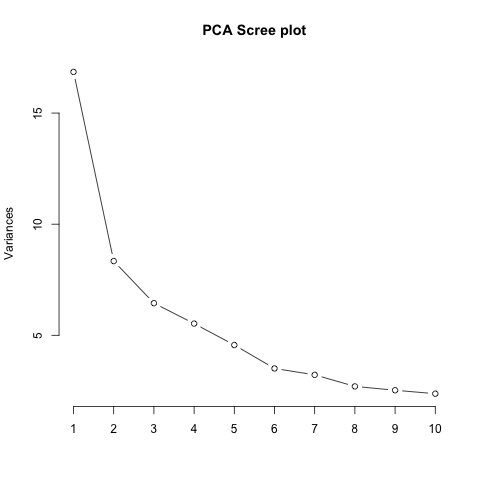
\includegraphics[width =  6cm, height = 6cm]{../images/model_pca_scree_plot.png}
      \caption{PCA scree plot for each principal component}
      \label{figurelabel}
   \end{figure}

After removing near zero variance 519 to 128. This indicates that a great number of predictors have apporiximately identical across observations. Figure 4 shows a PCA scree plot for each principal component. It indicates that first few principal components effectively explain the variances of data, and overall graph exponentially decays. Cumulative Proportion in $Table model_pca$ shows that first 10 pcs and 61 pcs explain approximately 44\% and 90\% of variance in dataset respectively. It means that if we decide to reduce dimensionality at the expense of a bit little of prediction accuracy, we could use 61 principal components which are approximately 1/8 of total predictors. 

   \begin{figure}[thpb]
      \centering
      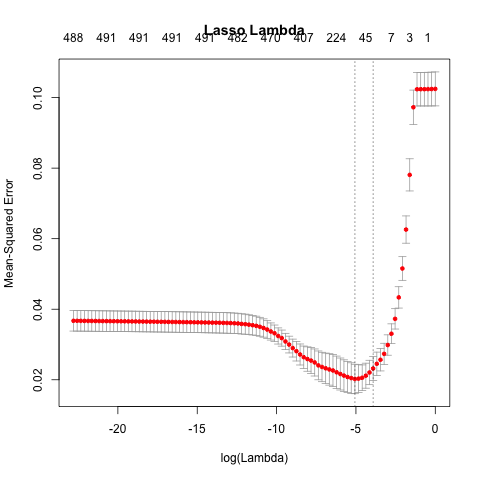
\includegraphics[width =  4cm, height = 4cm]{../images/model_lasso_lambda.png}
      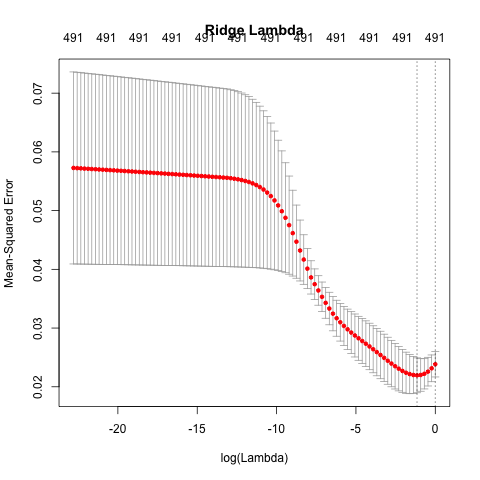
\includegraphics[width =  4cm, height = 4cm]{../images/model_ridge_lambda.png}
      \caption{MSE values for Lambda Values - Lasso Regression (left) and Ridge Regression (right)}
      \label{figurelabel}
   \end{figure}

Furthermore, we try to fit both lasso and regression and tune lambda values using 5-fold cross validation and then examine coefficients. Figure 5 shows respectively the Mean Square Error for corresponding lambda values for both models. The Figure suggests that MSE decreases as log(lambda) increase up to log lambda equals -5 and  -1.15 respectively. Based on these results, we decide optimal lambda for both model. 

   \begin{figure}[thpb]
      \centering
      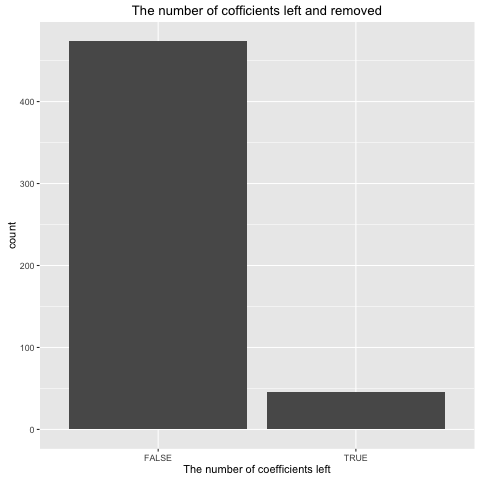
\includegraphics[width =  7cm, height = 6cm]{../images/model_lasso_number_of_coefficients_left.png}
      \caption{Number of Coefficients - Lasso Regression}
      \label{figurelabel}
   \end{figure}

We also examine coefficients of lasso regression. Figure 6 indicates that most of weights for corresponding predictors become zeros, which effectively eliminates a great portion of predictors. After elimination, only 78 predictors are left. We plot top 10 coefficients for both lasso and ridge to investigate how much each coefficient contribution to the model. 

   \begin{figure}[thpb]
      \centering
      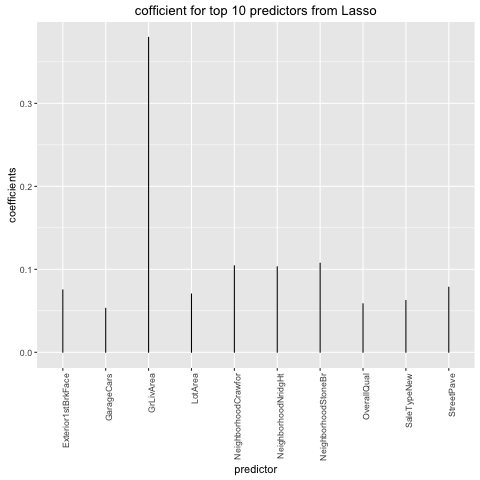
\includegraphics[width =  4cm, height = 4cm]{../images/model_lasso_coefficients_top_10.png}
      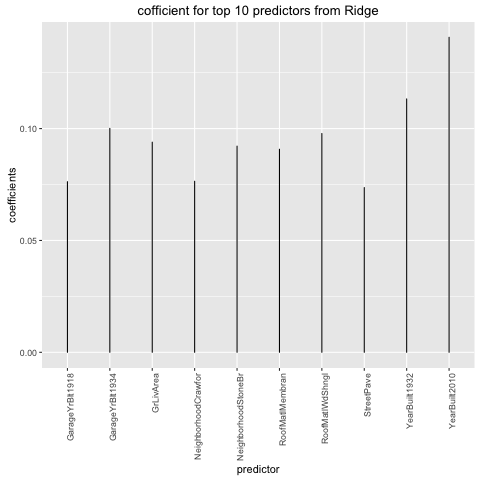
\includegraphics[width =  4cm, height = 4cm]{../images/model_ridge_coefficients_top_10.png}
      \caption{Top 10 Coefficients - Lasso Regression (left) and Ridge Regression (right)}
      \label{figurelabel}
   \end{figure}

Figure 7 shows the top 10 coefficients from both models. It is noteworthy that GrivArea has the highest coefficient in Lasso and YearBuilt2010 has the highest coefficient in Ridge. Both make sense because the area and built year are important aspects when it comes to making a decision about purchasing house. Both models indicate that GrLiArea, NeighborhoodCrawfor and NeighborhoodStoneBr belong to top 10 highest coefficients and are highly associated with house price. Furthermore, we try to figure out feature importance using Gradient boosting machine. Feature importance is automatically measured as GBM grows its tree while minimizing entropy. Figure $model_gbm_predictor importance.png$ shows that overall quality has the highest feature importance 

\section{RESULTS}

As a result, Figure 8 shows model comparison between true price and predicted price. 

   \begin{figure}[thpb]
      \centering
      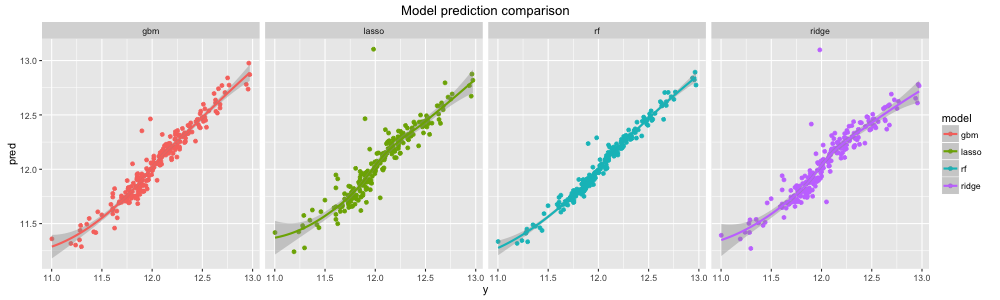
\includegraphics[width =  9cm, height = 4cm]{../images/model_prediction_comparison.png}
      \caption{Model Comparison between True Price and Predicted Price}
      \label{figurelabel}
   \end{figure}

Four models are fairly accurate and most of data points are located on diagonal line, which indicates a strong linear relationship between true price and predicted. Especially, Random Forest is especially well fitted among these four. 

   \begin{figure}[thpb]
      \centering
      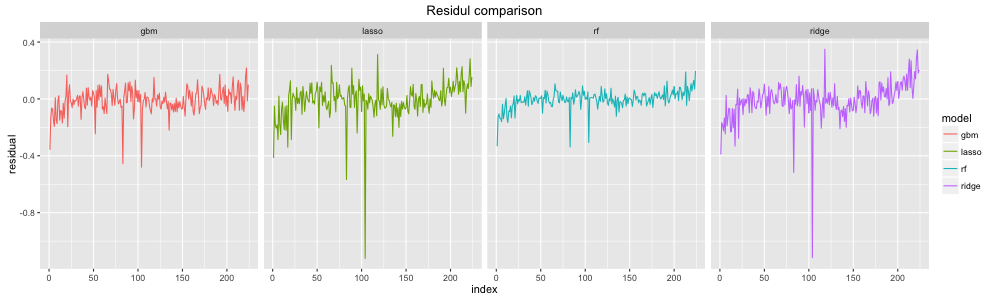
\includegraphics[width =  9cm, height = 4cm]{../images/model_residual_comparison.png}
      \caption{Model Comparison - Residual Plots of Four Models}
      \label{figurelabel}
   \end{figure}

Figure 9 shows the residual plots for four models. The residual is the difference between real house price and predicted price from models. We can see from Figure 9 that all models overestimate the price for cheaper house and underestimate the price for expensive house. This phenomenon is not surprising because we have few data points in cheapest and most expensive houses. Thus, the models incur a high bias in these end zones. This can be alleviated if we gather more data if possible. Compared to Lasso and Ridge, Gradient boosting machine and Random Forest are more stable. Both Lasso and Ridge have huge errors in the middle of graphs. 

Lastly, Table 2 as below shows RMSLE for each model, which is measured from hold-out dataset. It indicates that Random Forest predicts target variable the best.

% latex table generated in R 3.2.3 by xtable 1.8-2 package
% Mon Dec  5 17:32:43 2016
\begin{table}[ht]
\centering
\begin{tabular}{rrl}
  \hline
 & RMSLE & model \\ 
  \hline
1 & 0.06 & RandomForest \\ 
  2 & 0.08 & GBM \\ 
  3 & 0.13 & Ridge \\ 
  4 & 0.13 & Lasso \\ 
   \hline
\end{tabular}
\caption{Table 2: RMSEL Comparison from Four Models} 
\end{table}


\section{CONCLUSIONS}

In conclusions, while participating in the Kaggle competition - "House Price: Advanced Regression Techniques", we get a chance to dig down into real-life dataset that have complicated variables, missing values and large number of data entries. Based our analysis on the train dataset, we try to find the regression model and advanced techniques that most accurately predict the housing price, and use the exact model to predict new entries from test file. Exploring and creating visualization of data, we compare the usage of different regression models to understand the relationship between dependent variable SalePrice and 79 potential predictors. Fortunately, we ranked No.10 among all 2000 participating teams with our prediction, which not only shows the precision of our own predictive model, but also suggests room of improvement and growth.

This course gives us great opportunity to practice project reproducibility, advanced statistical model learning and teamwork delegation. By deligating work to each team mate and implementing the model to generate results, we aim to maintain project reproducibility and publicity so that more people can learn from our model and benefit for future researches. If you have any questions or concerns regarding any part of our analysis, please feel free to contact the authors for further clarification.

\addtolength{\textheight}{-12cm} 

\section*{ACKNOWLEDGMENT}

The Ames Housing dataset was compiled by Dean De Cock for use in data science education. It's an incredible alternative for data scientists looking for a modernized and expanded version of the often cited Boston Housing dataset.

\begin{thebibliography}{99}

\bibitem{c1} L1 vs. L2 Loss Function from Rishy Github: http://rishy.github.io/ml/2015/04/28/l1-vs-l2-loss/
\bibitem{c2} Root Mean Squared Logarithmic Error, https://www.kaggle.com/wiki/RootMeanSquaredLogarithmicError
\bibitem{c3} Handbook: General principles for dealing with missing data: https://goo.gl/G54nBx
\bibitem{c4} data-description.txt from Kaggle Competition: https://goo.gl/XGyi7m
\bibitem{c5} Log Transformation Standard: http://onlinestatbook.com/2/\newline
transformations/log.html
\bibitem{c6} One-hot, Wikipedia: https://en.wikipedia.org/wiki/One-hot
\bibitem{c7} The Elements of Statistical Learning, Shrinkage methods p.61  p. 305 
\bibitem{c8} Y. Bengio; A. Courville; P. Vincent (2013). "Representation Learning: A Review and New Perspectives". IEEE Trans. PAMI, special issue Learning Deep Architectures. 35: 1798–1828. doi:10.1109/tpami.2013.50.
\bibitem{c9} An Open Letter to Yann LeCun - Small Data requires Specialized Deep Learning: https://medium.com/@ShaliniAnanda1/an-open-letter-to-yann-lecun-22b244fc0a5a\#.92x0bez05
\bibitem{c10} "What is the intuitive explanation of feature engineering in machine learning? - Quora". www.quora.com. Retrieved 2015-11-11.
\bibitem{c11} Ensemble learning, http://www.scholarpedia.org/article/Ensemble\_learning
\bibitem{c12} Random forest, https://www.stat.berkeley.edu/~breiman/randomforest2001.pdf
\bibitem{c13} Principal component analysis: https://en.wikipedia.org/wiki/ \newline
Principal\_component\_analysis

\end{thebibliography}

\end{document}
